\documentclass[11pt]{article}
\usepackage[T1]{fontenc}
\usepackage{lmodern}
\usepackage[margin=1.05in]{geometry}
\usepackage{amsmath,amssymb,amsthm,mathtools}
\usepackage{booktabs,array,longtable}
\usepackage{microtype}
\usepackage{xcolor}
\usepackage{tikz}
\usetikzlibrary{arrows.meta,positioning}
\usepackage{xurl}
\usepackage{flafter}
\usepackage{placeins}
\usepackage[hidelinks]{hyperref}
\usepackage{bookmark}
\DeclareMathOperator{\Tr}{Tr}
\DeclareMathOperator{\diag}{diag}
\newcommand{\Id}{I}
\newcommand{\R}{\mathbb R}
\newcommand{\C}{\mathbb C}
\newcommand{\N}{\mathbb N}
\newcommand{\norm}[1]{\lVert#1\rVert}
\newcommand{\abs}[1]{\lvert#1\rvert}
\newtheorem{theorem}{Theorem}[section]
\newtheorem{proposition}[theorem]{Proposition}
\newtheorem{lemma}[theorem]{Lemma}
\newtheorem{corollary}[theorem]{Corollary}
\theoremstyle{remark}
\newtheorem{remark}[theorem]{Remark}
\numberwithin{equation}{section}
\setlength{\emergencystretch}{1em}
\title{A boundary-field gap for the spin-one Heisenberg chain}
\author{OpenAI}
\date{September 24, 2026}
\hypersetup{pdftitle={A boundary-field gap for the spin-one Heisenberg chain},pdfauthor={OpenAI}}
\pdfinfoomitdate=1
\pdftrailerid{}
\pdfsuppressptexinfo=15
\begin{document}
\maketitle
\begin{abstract}
We prove a uniform spectral gap for odd open spin-one antiferromagnetic
Heisenberg chains with the same fixed magnetic field at both endpoints.
The field $h=3/5$ gives a gap greater than $\log(10)/392$ on every chain
of $2L+1$ sites with $L\ge960$. Tasaki's index theorem then gives index $-1$
for every subsequential local limit of these boundary-selected ground states.
\end{abstract}

\section{Introduction}
Equal positive magnetic fields at the endpoints of an odd open spin-one
Heisenberg chain select a unique finite-volume ground state
\cite[Lemma 1]{Tasaki2025}. The remaining question is whether the
excitation gap stays positive as the chain grows. We prove a
quantitative gap for one fixed field in the pure bilinear model.
This is the boundary formulation used by Tasaki to connect the
Haldane gap problem to a nontrivial topological index \cite{Tasaki2025}.

In the orthonormal basis $e_m$, $m=-1,0,1$, of $\C^3$, let
\[
 S^ze_m=me_m,\qquad
 S^+e_m=\sqrt{2-m(m+1)}\,e_{m+1}\quad(m<1),\qquad S^+e_1=0,
\]
and put $S^-=(S^+)^*$, $S^x=(S^++S^-)/2$, and
$S^y=(S^+-S^-)/(2i)$. Thus $\sum_\alpha(S^\alpha)^2=2\Id$.
For $L\ge1$ and $h>0$, consider the operator on
$(\C^3)^{\otimes(2L+1)}$ given by
\begin{equation}\label{eq:target}
 H_L(h)=\sum_{j=-L}^{L-1}\sum_{\alpha=x,y,z}S_j^\alpha S_{j+1}^\alpha
       -h(S_{-L}^z+S_L^z).
\end{equation}
There is no bond between the endpoints. Write $E_0(L,h)\le E_1(L,h)$
for its two lowest eigenvalues, counted with multiplicity. We address
the fixed-boundary-field gap assertion: for some single $h>0$, the
difference $E_1(L,h)-E_0(L,h)$ stays bounded away from zero as
$L\to\infty$.

\begin{theorem}\label{thm:main}
For the Hamiltonian \eqref{eq:target}, with the spin normalization above,
\[
 E_1(L,3/5)-E_0(L,3/5)>\frac{\log 10}{392}
 \qquad\text{for every integer }L\ge960.
\]
\end{theorem}

\paragraph{Context and prior work.}
Haldane's prediction, formulated in 1981 and published in 1983,
distinguishes integer and half-odd-integer isotropic antiferromagnetic
Heisenberg chains, with a positive bulk gap for positive integer spin
\cite{Haldane1981,Haldane1983PLA,Haldane1983PRL}.
For spin one-half, Lieb, Schultz and Mattis had already constructed
excitations of the periodic chain whose energy above the ground state
vanishes with its length \cite[Appendix B]{LSM1961}.
The Affleck--Kennedy--Lieb--Tasaki construction gave a rigorous gapped
spin-one model \cite{AKLT1987,AKLT1988}. Its interaction contains a
biquadratic term: with $q=\mathbf S_j\cdot\mathbf S_{j+1}$, it is
proportional to $q+q^2/3$ up to an additive constant. Our Hamiltonian
has the pure bilinear interaction $q$ and fixed endpoint fields.

The endpoint condition matters even when the bulk interaction is
fixed. White and Huse numerically characterized the effective
spin-one-half degrees of freedom at free ends \cite{WhiteHuse1993}.
To estimate bulk properties, including the gap, they added physical
spin-one-half endpoint sites and adjusted their couplings. Magnetic
fields on the original spin-one endpoints give a different
finite-volume model, whose gap requires its own boundary estimates.

Tasaki formulated precisely this boundary problem in his work on the
topological character of the spin-one Heisenberg ground state
\cite{Tasaki2025}. Equation (2) of that paper is the Hamiltonian
\eqref{eq:target}; Lemma 1 proves uniqueness for every $L\ge1$ and
$h>0$. Assumption 2 asks for a positive gap uniform in all sufficiently
large $L$, at one fixed $h>0$. Theorem~\ref{thm:main} resolves this
fixed-boundary-field Haldane gap assertion positively and establishes
that assumption. Section~\ref{sec:topology} then derives Tasaki index
$-1$ for every boundary-selected subsequential local limit.

The topological viewpoint developed through several distinct
descriptions. Den Nijs and Rommelse introduced nonlocal string order
\cite{DenNijsRommelse1989}, and Kennedy and Tasaki connected it to
hidden symmetry breaking \cite{KennedyTasaki1992}. Pollmann, Turner,
Berg and Oshikawa described symmetry protection through matrix-product
states and the entanglement spectrum \cite{Pollmann2010}; Ogata
extended the bond-centered reflection index to infinite-chain states
beyond the matrix-product description \cite{Ogata2021}.
Tasaki's local-twist index \cite{Tasaki2018} instead uses the twist
expectation studied by Nakamura and Todo \cite{NakamuraTodo2002}.
The boundary-state theorem in \cite{Tasaki2025} uses uniform $z$
rotations and site-centered reflection. These invariances imply
invariance under site reflection combined with a global $\pi$ rotation
about $z$, the symmetry studied by Fuji, Pollmann and Oshikawa
\cite{FujiPollmannOshikawa2015}.
Our consequence concerns Tasaki's index in this precise symmetry
setting; it does not identify the different diagnostics above.

\paragraph{Methodological inputs.}
For frustration-free chains, Lemm and Mozgunov proved finite-size
criteria involving both interior and boundary-segment gaps
\cite{LemmMozgunov2019}. Here the boundary information comes from
weighted spatial moments and a coupled Gibbs-purity recurrence.
The finite trial vectors use the matrix-product framework of finitely
correlated states \cite{FNW1992} and its finite-chain formulation
\cite{PerezGarcia2007}; they certify energy upper bounds that
initialize the recurrence.

The continuous-history representation is an instance of the
time-ordered Poisson expansion of Aizenman and Nachtergaele
\cite{AizenmanNachtergaele1994}. The particular spatial transfer
operator and finite periodic estimates used here come from
\cite{periodic}, which proves a uniform gap on even periodic rings.
We retain that source's spin normalization, coupling, and energy
shift, and state explicitly the transfer and finite-input results
used below. The endpoint pairings and all estimates specific to the
open chain are proved here.


\paragraph{Proof strategy.}
For each inverse temperature $b>0$, a partition function of the
periodic model is a trace of a power of a compact self-adjoint spatial
operator $X_b$. For the open chain with \emph{opposite} endpoint fields,
the corresponding partition function is instead a boundary pairing
$\langle v_b,X_b^n v_b\rangle$, where $n$ is the number of sites.
At even $n$, this is a positive weighted moment of the absolute spatial
eigenvalues. A rotation of the right boundary vector produces the
same-field Hamiltonian in \eqref{eq:target}.

The periodic estimates show that one spatial eigenvalue dominates
sufficiently high even moments. For the open chain, however, the contribution of
each eigenspace is weighted by its overlap with $v_b$, and this vector
changes with temperature. Periodic concentration therefore leaves a
boundary-overlap problem. We solve it by contracting the residual
boundary-weighted moments while tracking the physical Gibbs
purity (the sum of the squared Gibbs probabilities) of the opposite-field
chain. These two estimates improve together
when both length and inverse temperature double, without assuming a
nonzero boundary overlap at the next temperature. Once the leading
spatial line dominates the boundary pairing, its rotation invariance
controls the same-field expression at every odd length in a full
dyadic interval. The purity defect then decreases at a rate exponential
in the inverse temperature, which yields a uniform physical gap.

Sections~\ref{sec:transfer} and \ref{sec:periodic} establish the transfer
representation and the periodic estimates in the form needed here.
Section~\ref{sec:boundary} proves the boundary recurrence.
Section~\ref{sec:initialization} initializes and iterates it, and
Section~\ref{sec:conclusion} proves Theorem~\ref{thm:main} at all the
required odd lengths. Section~\ref{sec:topology} applies the resulting
gap to the boundary-selected infinite-volume states.
Appendices~\ref{app:thermal} and \ref{app:trials}
give complete finite certificates for the boundary initialization.
All terminating decimals used in inequalities denote exact rationals.

\section{Spatial transfer with endpoint fields}\label{sec:transfer}
We first put the periodic and open chains in the same transfer
representation. The boundary vectors, including their complex phases,
will distinguish the physical endpoint fields.
The time-ordered bond expansion has a general formulation in
\cite[arXiv v1, Section 2.2, Equations (2.10)--(2.12)]{AizenmanNachtergaele1994}.
We prove the required boundary identity directly with the specified
kernel and field coefficients.

\subsection{Hamiltonians and shifted partition functions}
From now on set
\begin{equation}\label{tr:constants}
 h=\frac35,\qquad a=\frac{700741}{500000},\qquad
 b_0=\frac{49}{4},\qquad b_j=2^jb_0\quad(j\ge0).
\end{equation}
It is convenient to label an $n$-site chain by $0,\ldots,n-1$.
Write $S_j\cdot S_k=\sum_\alpha S_j^\alpha S_k^\alpha$ and define
\begin{align}
 H_n^{\rm opp}&=\sum_{j=0}^{n-2}S_j\cdot S_{j+1}
                         -hS_0^z+hS_{n-1}^z,\label{tr:Hopp}\\
 H_n^{\rm s}&=\sum_{j=0}^{n-2}S_j\cdot S_{j+1}
                         -hS_0^z-hS_{n-1}^z,\label{tr:Hsame}\\
 H_n^{\rm per}&=\sum_{j=0}^{n-2}S_j\cdot S_{j+1}
                         +S_{n-1}\cdot S_0\quad(n\ge4).
\end{align}
For $n=2L+1$, $H_n^{\rm s}$ is \eqref{eq:target} after relabeling.
Our partition functions are ordinary traces over the entire physical
Hilbert space:
\begin{equation}\label{tr:partitions}
 \begin{split}
 Z_n(b)&=\Tr e^{-b(H_n^{\rm per}+an\Id)},\\
 Y_n(b)&=\Tr e^{-b(H_n^{\rm opp}+an\Id)},\qquad
 Y_n^{\rm s}(b)=\Tr e^{-b(H_n^{\rm s}+an\Id)}.
 \end{split}
\end{equation}
The shift is per site, also for open chains. It will cancel from all
physical Gibbs weight ratios.

\subsection{The spatial operator}
We use the concrete spatial-transfer operator in
\cite[Proposition 3.1]{periodic}. Its auxiliary space records ordered
bond events in imaginary time; each physical site contributes a kernel
depending on its two incident histories. Use the unitarily equivalent
Cartesian
spin matrices $(S^\alpha)_{rs}=-i\varepsilon_{\alpha rs}$ and set
$G_\alpha=iS^\alpha$. Then $G_\alpha$ is real,
$\norm{G_\alpha}=1$, and
\[
 -S\cdot S=\sum_{\alpha=x,y,z}G_\alpha\otimes G_\alpha.
\]
A history is an ordered list
$\omega=((t_1,\alpha_1),\ldots,(t_d,\alpha_d))$ with
$0<t_1<\cdots<t_d<b$ and $\alpha_r\in\{x,y,z\}$; the empty list
is allowed. Give the disjoint union $\Omega_b$ of these labeled
simplexes Lebesgue measure on each simplex and mass one at the empty
history. Its measure $\mu_b$ has total mass $e^{3b}$.

For two histories, merge their events in chronological order and take
the trace of the resulting product of $G$ matrices, with increasing
time from left to right. Denote this real kernel by $k_b(\omega,\eta)$.
Set it to zero at nonempty time
collisions, a null set, and use trace $3$ for the two empty histories.
The kernel is symmetric: exchanging the two histories leaves their
merged list unchanged. In particular, symmetry does not reverse a
product of noncommuting matrices. Moreover $|k_b|\le3$.
On $\mathcal K_b=L^2(\Omega_b,\mu_b;\C)$ define
\begin{equation}\label{tr:operator}
 (X_bf)(\omega)=e^{-ab}\int_{\Omega_b}k_b(\omega,\eta)
                                      f(\eta)\,d\mu_b(\eta).
\end{equation}
It is real, self-adjoint, and Hilbert--Schmidt. The cited transfer
Proposition identifies its periodic moments:
\begin{equation}\label{tr:periodic}
 Z_n(b)=\Tr X_b^n\quad(n\ge4),\qquad
 \sum_i|\mu_i(b)|^k<\infty\quad(k\ge2),
\end{equation}
where $\mu_i(b)$ lists its nonzero eigenvalues with multiplicity.
This exact operator, with the shift in \eqref{tr:constants}, is the one
used for the periodic inputs in Section~\ref{sec:periodic}.

Rotations will let us change one endpoint field and, later, show that
the leading spatial line is fixed. Let $D_2$ consist of the identity
and the three diagonal rotations by
$\pi$, let $C$ cyclically permute the coordinate axes, and put
$\mathcal G=\langle D_2,C\rangle$. This is a group of twelve proper
signed permutations. If $ge_\alpha=\epsilon_g(\alpha)
e_{\sigma_g(\alpha)}$, write $\sigma_g\omega$ for relabeling the
marks and $s_g(\omega)=\prod_r\epsilon_g(\alpha_r)$. The operators
\begin{equation}\label{tr:rotations}
 (U_gf)(\omega)=s_g(\sigma_g^{-1}\omega)f(\sigma_g^{-1}\omega)
\end{equation}
form a real unitary representation and commute with $X_b$. This follows
either directly by rotating every matrix in the kernel, or from the
same Proposition. In particular, fix
$P=\diag(1,-1,-1)$, so $Pe_z=-e_z$.

\subsection{Boundary vectors}
Define $v_b\in\mathcal K_b$ by
\begin{equation}\label{tr:vector}
 v_b(\omega)=
 \begin{cases}
 (ih)^d,&\text{all $d$ marks of $\omega$ equal $z$},\\
 0,&\text{otherwise}.
 \end{cases}
\end{equation}
The empty-history value is one. The simplex volumes give
$\norm{v_b}^2=\sum_{d\ge0}b^dh^{2d}/d!=e^{bh^2}$.
The inner product below is conjugate linear in its first argument.

\begin{proposition}[Open-chain transfer]\label{tr:boundary}
For $b>0$, $n\ge2$, and $g\in\mathcal G$, the pairing
$\langle v_b,X_b^nU_gv_b\rangle$ is the shifted partition function
of the open chain with left field $-hS_0^z$ and right field
$+hS_{n-1}^{ge_z}$. Consequently
\begin{equation}\label{tr:open}
 Y_n(b)=\langle v_b,X_b^nv_b\rangle,\qquad
 Y_n^{\rm s}(b)=\langle v_b,X_b^nU_Pv_b\rangle.
\end{equation}
Here $S^u=\sum_\alpha u_\alpha S^\alpha$ for a real vector $u$.
\end{proposition}
\begin{proof}
Expand the negative Hamiltonian exponential into its ordered-time
series. Each bond event inserts two $G_\alpha$ matrices, by the
Cartesian identity above. At the left endpoint, the conjugated
coefficient in \eqref{tr:vector} gives
$(-ih)G_z=+hS^z$ per event; at the right endpoint the coefficient is
$(ih)G_z=-hS^z$. Relabeling by $g$ and multiplying its signs changes
this last insertion to $-hS^{ge_z}$. These are exactly the two field
insertions in the negative Hamiltonian stated in the Proposition.

Regroup the series by the boundary histories $\omega_0,\omega_n$
and the $n-1$ bond histories $\omega_1,\ldots,\omega_{n-1}$.
Their interleavings partition each full time simplex up to null
collisions. At site $r$, $0\le r<n$, the trace is
$k_b(\omega_r,\omega_{r+1})$, in the original chronological order.
Integrating these $n$ kernel factors against the two boundary
coefficients gives $X_b^n$ and the shift factor $e^{-ban}$.
No bond joins the endpoints.

This regrouping is legitimate: the absolute sum of traced terms is
bounded by
$3^n\exp\{b[3(n-1)+2h]\}$ before the scalar shift. All sums and
integrals are therefore absolutely convergent. Choosing $g=1$ and
$g=P$ gives \eqref{tr:open}.
\end{proof}

\begin{figure}[!htbp]
\centering
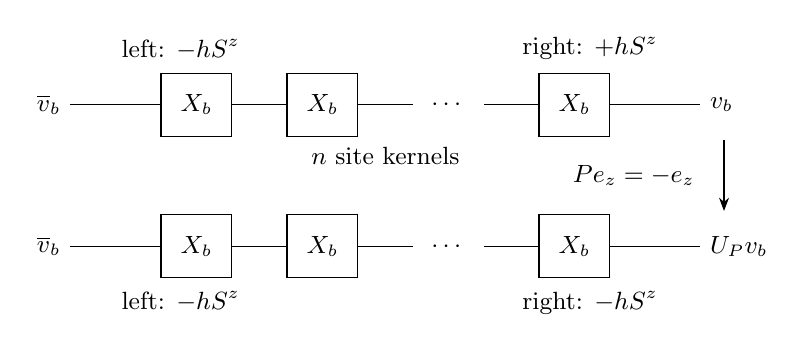
\begin{tikzpicture}[>=Stealth,
  site/.style={draw,minimum width=9mm,minimum height=8mm},
  every node/.style={font=\small}]
 \foreach \y in {0,-1.8} {
   \node[site] at (0,\y) {$X_b$};
   \node[site] at (1.6,\y) {$X_b$};
   \node at (3.2,\y) {$\cdots$};
   \node[site] at (4.8,\y) {$X_b$};
   \draw (-1.6,\y)--(-.45,\y);
   \draw (.45,\y)--(1.15,\y);
   \draw (2.05,\y)--(2.75,\y);
   \draw (3.65,\y)--(4.35,\y);
   \draw (5.25,\y)--(6.4,\y);
   \node[left] at (-1.6,\y) {$\overline v_b$};
 }
 \node[right] at (6.4,0) {$v_b$};
 \node[right] at (6.4,-1.8) {$U_Pv_b$};
 \node[above] at (-.2,.45) {left: $-hS^z$};
 \node[above] at (5.0,.45) {right: $+hS^z$};
 \node[below] at (-.2,-2.25) {left: $-hS^z$};
 \node[below] at (5.0,-2.25) {right: $-hS^z$};
 \draw[->] (6.7,-.45)--(6.7,-1.35);
 \node[left] at (6.45,-.9) {$P e_z=-e_z$};
 \node at (2.4,-.65) {$n$ site kernels};
\end{tikzpicture}
\caption{The two spatial boundary pairings. Each box contributes one
site kernel; the internal integrations represent the $n-1$ bonds.
Replacing the right boundary vector by $U_Pv_b$ changes the right
physical field. This is an identity between transfer representations,
not a claim that the two physical Hamiltonians are unitarily equivalent.}
\label{fig:boundary-pairings}
\end{figure}

For even lengths, the opposite-field expression is the positive moment
$Y_n(b)=\langle v_b,|X_b|^n v_b\rangle$.
At odd lengths, the powers of $X_b$ retain the signs of its eigenvalues.
We first concentrate the even opposite-field moments. The resulting
leading-line estimate will then control the signed same-field pairing
at odd lengths; Figure~\ref{fig:boundary-pairings} distinguishes the
two boundary pairings.

\FloatBarrier
\section{Periodic concentration estimates}\label{sec:periodic}

The boundary argument requires quantitative information about the
spatial spectrum, including the change of its leading eigenvalue when
the inverse temperature doubles.  We extract that information from
finite periodic-chain estimates in~\cite{periodic}.  The extraction is
given in detail because the periodic gap theorem alone does not provide
these boundary estimates.  Throughout, terminating decimals denote
exact rational numbers, and eigenvalue lists count multiplicities.

For even $n\ge4$, put
\begin{equation}\label{per:purities}
 S(n,b)=\frac{Z_{2n}(b)}{Z_n(b)^2},\qquad
 T(n,b)=\frac{Z_n(2b)}{Z_n(b)^2}.
\end{equation}
The first is the purity of the spatial probabilities
$|\mu_i(b)|^n/Z_n(b)$, where $(\mu_i(b))$ is the nonzero spectrum of
$X_b$; the second is the purity of the physical Gibbs probabilities.
Both lie in $(0,1]$.  Doubling $n$ squares the first probability list,
whereas doubling $b$ squares the second.

\begin{lemma}[Squaring and concentration]\label{per:purity}
Let $(w_i)$ be a finite or countable probability list, and suppose its
purity is at least $1-u$, where $0\le u<1$.  Normalizing the squares
$w_i^2$ gives a list with purity defect at most
\begin{equation}\label{per:f}
 f(u)=\frac{u^2}{2(1-u)^2}.
\end{equation}
If $u<1/2$, the largest weight is unique and at least $1-u$.  Writing
$x$ for the sum of all the other weights, one has
\begin{equation}\label{per:concentration-elementary}
 x\le\frac{1-\sqrt{1-2u}}2.
\end{equation}
In particular, for $0\le u\le .1$,
\begin{equation}\label{per:d}
 \frac{x}{1-x}\le d(u),\qquad d(u)=\frac{u}{2-3u}.
\end{equation}
\end{lemma}

\begin{proof}
Set $P=\sum_iw_i^2$ and let $P'$ be the purity after squaring.
Nonnegativity justifies rearrangement of the countable sums, and
\[
 1-P'=\frac{2\sum_{i<k}w_i^2w_k^2}{P^2}
 \le\frac{2(\sum_{i<k}w_iw_k)^2}{P^2}
 =\frac{(1-P)^2}{2P^2}\le f(u).
\]
Here $f$ is increasing on $[0,1)$.  A summable nonzero nonnegative list
attains its maximum, and $P\le\max_iw_i$.  If $u<1/2$, the maximum
therefore exceeds $1/2$ and is unique.  Thus $x\le u<1/2$, and
\[
 2x(1-x)\le 1-P\le u,
\]
which gives~\eqref{per:concentration-elementary}.  Also
$x\le u/[2(1-x)]\le u/[2(1-u)]$; applying the increasing function
$x\mapsto x/(1-x)$ proves~\eqref{per:d}.
\end{proof}

For later reference we also record explicitly the interaction of the
two periodic purities.  This is \cite[Lemma 4.2]{periodic}; we include its short proof by
partition-function cancellation.

\begin{lemma}[Coupled update]\label{per:coupled}
Suppose that $n\ge4$ is even, $b>0$, and
$S(n,b)\ge s$, $T(2n,b)\ge t$, with $0<s,t\le1$.
Set
\[
 p_+=f(1-s^2t).
\]
If $p_+<1$, then
\begin{equation}\label{per:coupled-formula}
 1-S(2n,2b)\le p_+,\qquad
 1-T(4n,2b)\le f\bigl(1-t^2(1-p_+)\bigr).
\end{equation}
Either upper defect bound may be increased before subsequent use,
provided it stays below one.
\end{lemma}

\begin{proof}
Directly from~\eqref{per:purities},
\[
 S(n,2b)=S(n,b)^2\frac{T(2n,b)}{T(n,b)^2}
 \ge s^2t.
\]
Apply spatial squaring and Lemma~\ref{per:purity}.  A second cancellation
then gives
\[
 T(4n,b)=T(2n,b)^2\frac{S(2n,2b)}{S(2n,b)^2}
 \ge t^2(1-p_+).
\]
Physical squaring proves the second inequality.  Monotonicity of $f$
justifies increasing either defect bound.
\end{proof}

We next state the finite inputs gathered in the companion
\cite[Corollary 5.6]{periodic}. Its shift, spin normalization and unit
bilinear coupling are exactly those used here.
In particular, we use an intermediate row in the initialization proof,
not merely its final conclusion.

\begin{proposition}[Finite periodic inputs from~\cite{periodic}]
\label{per:native}
Set
\begin{equation}\label{per:constants}
 \ell=.999,\quad U=1.00139,\quad V=.872,\quad
 m_J=1.0657205,\quad m_N=.2783155.
\end{equation}
At $b_0=49/4$, the spatial eigenvalue list decomposes as one list $J$
and three identical lists $N$. Here $J$ is the spectrum on the subspace
fixed by every $U_g$, $g\in D_2$, and $N$ is the common spectrum on
each of the other three simultaneous eigenspaces of these commuting
operators.
In $J$ the absolute eigenvalues are at
most $U$, and their twelfth powers sum to at most $m_J$; in each $N$
they are at most $V$, and their twelfth powers sum to at most $m_N$.
There is an eigenvalue in $J$ whose modulus exceeds $\ell$.
Furthermore,
\begin{equation}\label{per:native-first-row}
 1-S(72,b_1)\le\frac{151249}{2500000}=.0604996.
\end{equation}
For the periodic chains of $72$ and $120$ sites, the shifted ground
energy is strictly negative.  Consequently, at each of these lengths
and every $b>0$, an individual unnormalized ground Boltzmann weight is
greater than one.
\end{proposition}

No boundary Hamiltonian occurs in Proposition~\ref{per:native}.
The finite periodic thermal and variational certificates supporting it
are given in the cited source.  We now deduce all the spatial estimates
that will be used for boundaries. The residual ratios will contract
the boundary-weighted tails. The upper and lower bounds comparing
successive leading eigenvalues will control the change of temperature
in the boundary concentration and physical-purity estimates,
respectively. Finally, positivity and rotation invariance of the
leading line will control the same-field pairing at odd lengths.

\begin{proposition}[Concentration at the doubling scales]
\label{per:concentration}
For every $j\ge0$, $X_{b_j}$ has a unique simple eigenvalue of largest
modulus.  This eigenvalue is positive; denote it by
$\lambda_j=\|X_{b_j}\|$.  Its eigenspace is fixed pointwise by
$\mathcal G$.  Let $\rho_j$ be the supremum of the absolute values of
all other eigenvalues divided by $\lambda_j$.  Then
\begin{equation}\label{per:initial-ratios}
 \ell<\lambda_0\le U,\qquad
 \rho_0<.874,\qquad \rho_1<.9525,\qquad \rho_2<.971.
\end{equation}
For $j\ge2$, define
\begin{equation}\label{per:scales}
 n_j=120\,2^{j-2},\qquad M_j=2n_j,\qquad
 u_2=.052,\qquad u_{j+1}=6u_j^2.
\end{equation}
The following bounds hold for every $j\ge2$:
\begin{align}
 1-S(n_j,b_j)&\le u_j,&
 1-T(M_j,b_j)&\le u_j, \label{per:tracked-purities}\\
 \rho_j^{n_j}&\le d(u_j). &&\label{per:spectral-ratio}
\end{align}
Finally, put $r_j=\lambda_{j+1}/\lambda_j^2$.  Then
\begin{equation}\label{per:lambda-ratios}
 0<r_j\le1\quad(j\ge0),\qquad
 r_j^{M_j}\ge(1-u_j)(1-u_{j+1})\quad(j\ge2).
\end{equation}
\end{proposition}

\begin{proof}
Until positivity has been proved, write $\lambda_j=\|X_{b_j}\|$ for
the maximal spectral modulus.

\emph{The initial spatial spectrum.}
Remove an eigenvalue in $J$ whose modulus exceeds $\ell$.
The remaining twelfth-power mass in $J$ is at most
$m_J-\ell^{12}<\ell^{12}$, while $V<\ell$ bounds each of the other
three sectors.  The removed eigenvalue is therefore the unique simple
eigenvalue of maximal modulus.  The exact rational inequalities
\[
 m_J-\ell^{12}<(.874\ell)^{12},\qquad V<.874\ell
\]
prove $\rho_0<.874$.

We need the total residual moments as well as this individual ratio
bound.  For every real $k\ge12$, define
\begin{equation}\label{per:D}
 D(k)=\frac{(m_J-\ell^{12})^{k/12}
       +3\bigl[V^k+(m_N-V^{12})^{k/12}\bigr]}{\ell^k}.
\end{equation}
The sum of the $k$th powers of all nondominant absolute eigenvalue
ratios at $b_0$ is at most $D(k)$.  Indeed,
$V^{12}<m_N<2V^{12}$; for a nonnegative list with entries at most
$V^{12}$ and total mass at most $m_N$, convexity of $x^{k/12}$ bounds
the sum by $(V^{12})^{k/12}+(m_N-V^{12})^{k/12}$.  This follows by
moving mass to fill one entry before the next; finite sublists followed
by a limit give the countable case.  Without an entry cap, the
corresponding bound is simply the total mass to the power $k/12$.
Applying these facts to the four sectors proves the claim.  In
particular, for even $k\ge12$,
\begin{equation}\label{per:Z-initial}
 Z_k(b_0)\le U^k(1+D(k)).
\end{equation}

\emph{Reseeding at $(120,b_2)$.}
Our next goal is to make both $1-S(120,b_2)$ and $1-T(240,b_2)$
at most $.052$, so that one quadratic recurrence will control them.
A coupled update will give these bounds from spatial and physical
seeds at $(60,b_1)$ and $(120,b_1)$, respectively. To obtain the
spatial seed, we combine a leading-eigenvalue lower bound from length
$72$ with a residual-moment upper bound at length $32$, then increase
the moment order to $60$. The same residual estimate also supplies
the ratio $\rho_1$ needed in the first boundary updates.

By~\eqref{per:native-first-row} and Lemma~\ref{per:purity}, the spatial
list at $(72,b_1)$ has a unique largest weight.  Thus $X_{b_1}$ also
has a unique simple eigenvalue of maximal modulus.  Moreover,
\[
 .0604996<2(.032)(.968)
\]
implies that this weight exceeds $.968$.  The periodic trial at length
$72$ gives $Z_{72}(b_1)>1$, so
\begin{equation}\label{per:lambda1}
 \lambda_1^{72}>.968.
\end{equation}
Physical squaring at length $32$ gives
$Z_{32}(b_1)\le Z_{32}(b_0)^2$.  Subtracting the dominant spatial
contribution and using~\eqref{per:Z-initial} and~\eqref{per:lambda1}
therefore yields
\begin{equation}\label{per:tail32}
 \sum_{i\ne0}\left|\frac{\mu_i(b_1)}{\lambda_1}\right|^{32}
 \le U^{64}(1+D(32))^2(.968)^{-32/72}-1
 <.9525^{32}.
\end{equation}
This proves $\rho_1<.9525$.  For any nonnegative list $(a_i)$ and
$q\ge p>0$, one has
$\sum_i a_i^q\le(\sum_i a_i^p)^{q/p}$ whenever the right side is finite.
Applying this to~\eqref{per:tail32} gives a residual $60$th moment below
$.9525^{60}$.  Retaining only the dominant term in the numerator of
$S(60,b_1)$ proves
\begin{equation}\label{per:seed-s}
 S(60,b_1)\ge s:=(1+.9525^{60})^{-2}.
\end{equation}

For the physical spectrum at length $120$, choose one ground
Boltzmann weight at $b_0$ and divide every other weight by it.
The chosen weight is greater than one by Proposition~\ref{per:native}.
Hence the sum of the other ratios is bounded above by
\[
 R=U^{120}(1+D(120))-1.
\]
When $b$ doubles, these ratios square, so their sum is at most $R^2$.
Keeping the chosen ground weight in the purity numerator now gives
\begin{equation}\label{per:seed-t}
 T(120,b_1)\ge t:=(1+R^2)^{-2}.
\end{equation}
This reasoning neither assumes ground-state simplicity nor discards
multiplicities.

Here are rational checks sufficient for every numerical comparison
just used and for the ensuing seed:
\begin{equation}\label{per:scalar-checks}
\begin{array}{rcl}
 D(32)&<&.0442,\\
 D(120)&<&.00000025,\\
 (.9856)^9&<&(.968)^4,\\
 U^{64}(1+.0442)^2/.9856-1&<&.2092<.9525^{32},\\
 s&>&.9002,\qquad t>.9372,\\
 f(1-.9002^2\,.9372)&<&.0502,\\
 f(1-.9372^2(1-.0502))&<&.0198.
\end{array}
\end{equation}
All comparisons are between explicit rational numbers after bounding
the cube roots in $D(32)$ by
\[
 (m_J-\ell^{12})^{1/3}<.426635,\qquad
 (m_N-V^{12})^{1/3}<.439736.
\]
Cubing verifies these two bounds; raising the bounds to the eighth
power gives the displayed bound on $D(32)$.  For $D(120)$ no roots
are needed.  The bound on $t$ follows already with
$D(120)$ replaced by $.00000025$.
Lemma~\ref{per:coupled}, applied to~\eqref{per:seed-s}--\eqref{per:seed-t}
at $(n,b)=(60,b_1)$, now gives
\[
 1-S(120,b_2)<.052,\qquad 1-T(240,b_2)<.052.
\]

\emph{Induction.}
For $0\le u\le .052$,
\begin{equation}\label{per:G}
 f\bigl(1-(1-u)^3\bigr)=G(u)u^2,\qquad
 G(u)=\frac12\left(\sum_{r=1}^3(1-u)^{-r}\right)^2.
\end{equation}
The function $G$ is increasing, and exact substitution gives
$G(.052)<5.583<6$.  Also $6u^2\le u$ on this interval.
Thus, if the two defects in~\eqref{per:tracked-purities} are at most
$u_j$, the first coupled output is at most $6u_j^2=u_{j+1}\le u_j$.
Using this upper bound in the second output bounds that output by the
same number.  This proves~\eqref{per:tracked-purities} for every
$j\ge2$.  Each spatial purity exceeds $1/2$, so the maximal spatial
modulus remains unique and simple.  Applied to its probability list,
Lemma~\ref{per:purity} also gives
\[
 \sum_{i\ne0}\left|\frac{\mu_i(b_j)}{\lambda_j}\right|^{n_j}
 \le d(u_j),
\]
which proves~\eqref{per:spectral-ratio}.
The rational comparison $d(.052)<.971^{120}$ gives $\rho_2<.971$.

\emph{The sign and the rotation symmetry.}
At every level we have proved uniqueness of the eigenvalue of maximal
modulus.  If it were $-\lambda_j$, then
$\Tr(X_{b_j}^n)/\lambda_j^n$ would tend to $-1$ through odd integers
$n$.  Indeed, the residual ratios are bounded by some number below one,
and their fourth powers have finite sum, so their $n$th-power sum
vanishes as $n\to\infty$.  This contradicts the strictly positive
physical partition function $Z_n(b_j)$ at odd $n\ge5$.
The leading eigenvalue is therefore $+\lambda_j$.

Its eigenspace has a real unit vector, since $X_{b_j}$ is real.
The real unitaries $U_g$ commute with $X_{b_j}$, so they act on that
line by signs.
The order-three cyclic rotation $C$ must act by $+1$.  It conjugates
the three nonidentity elements of $D_2$ cyclically, so they have the
same sign on the line.  Since the product of any two is the third,
that common sign equals its square and hence is $+1$.
Thus every element of $\mathcal G=\langle D_2,C\rangle$ fixes the
leading eigenspace pointwise.

\emph{Comparing the leading eigenvalues.}
For every even $N\ge4$, physical squaring gives
$Z_N(b_{j+1})\le Z_N(b_j)^2$. The residual-tail estimate used above
gives $Z_N(b_j)/\lambda_j^N=1+o(1)$, so
$Z_N(b_j)^{1/N}\to\lambda_j$. Taking $N$th roots and letting $N$
tend to infinity through even integers therefore yields
$\lambda_{j+1}\le\lambda_j^2$.
For the opposite direction at the reference scale, recall that
$M_j=n_{j+1}$.  The leading spatial probability at $(M_j,b_{j+1})$
is at least $1-u_{j+1}$, so
\[
 \begin{split}
 \lambda_{j+1}^{M_j}
 &\ge(1-u_{j+1})Z_{M_j}(b_{j+1})\\
 &= (1-u_{j+1})T(M_j,b_j)Z_{M_j}(b_j)^2\\
 &\ge(1-u_{j+1})(1-u_j)\lambda_j^{2M_j}.
 \end{split}
\]
This proves~\eqref{per:lambda-ratios} and completes the proof.
\end{proof}

\section{Concentration of boundary-weighted moments}\label{sec:boundary}
We now pass from unweighted spatial traces to the boundary pairing for
the opposite-field chain. We will control two quantities together: the
fraction of an even boundary moment outside the leading spatial line,
and the defect of the physical Gibbs purity. The boundary coefficients
depend on temperature. We compare the weighted moments across temperatures
through physical partition-function identities, while contracting the
residual spatial powers at a fixed temperature.

Use the simple positive leading eigenvalue $\lambda_j$ and residual
ratio $\rho_j$ from Section~\ref{sec:periodic}. Let $P_j$ be the
orthogonal projection onto its line, and put
\begin{equation}\label{be:definitions}
 \begin{split}
 c_j&=\norm{P_jv_{b_j}}^2,\\
 B_k(j)&=\langle v_{b_j},(|X_{b_j}|/\lambda_j)^k v_{b_j}\rangle,
 \qquad e_k(j)=\frac{B_k(j)-c_j}{B_k(j)},\\
 A(m,j)&=\frac{Y_m(b_{j+1})}{Y_m(b_j)^2}.
 \end{split}
\end{equation}
We use $k,m$ even and at least two. Then
$B_k(j)=Y_k(b_j)/\lambda_j^k>0$, so $e_k(j)$ is defined even if
$c_j=0$. Also $0\le e_k(j)\le1$ and $0<A(m,j)\le1$.
Thus $e_k(j)$ is the residual fraction of a spatial boundary moment,
whereas $A(m,j)$ is the physical Gibbs purity of the opposite-field
chain at inverse temperature $b_j$.

The normalized absolute spatial eigenvalues are at most one. Thus
$B_m(j)\le B_k(j)$ when $m\ge k$. More precisely, if
$D_k(j)=B_k(j)-c_j$, the spectral theorem gives
\begin{equation}\label{be:residual}
 0\le D_m(j)\le\rho_j^{m-k}D_k(j)\qquad(m\ge k).
\end{equation}
The powers act on the residual spectrum; no upper bound for the total
boundary norm is needed in this comparison.

\begin{lemma}[Transfer between temperatures]\label{be:recurrence}
Let $j\ge0$ and let $m>k\ge2$ be even. Suppose $e_k(j)<1$ and
$0<q<1$ with $q\ge\rho_{j+1}^{m-k}$. Define, for
$0\le e<1$ and $0<t\le1$,
\begin{equation}\label{be:F}
 F(q,e,t)=\frac{q}{1-q}\left(\frac{1}{(1-e)^2t}-1\right).
\end{equation}
Then
\begin{equation}\label{be:step}
 e_m(j+1)\le F(q,e_k(j),A(m,j)).
\end{equation}
In particular, an upper bound strictly below one on the right proves
$c_{j+1}>0$ without presupposing it.
\end{lemma}
\begin{proof}
At the new temperature, \eqref{be:residual} yields
$B_m(j+1)-c_{j+1}\le q[B_k(j+1)-c_{j+1}]$.
Subtract and rearrange to obtain
\[
 e_m(j+1)\le\frac{q}{1-q}
                   \left(\frac{B_k(j+1)}{B_m(j+1)}-1\right).
\]
Write $r_j=\lambda_{j+1}/\lambda_j^2$. From the definitions,
\begin{equation}\label{be:ratio}
 \frac{B_k(j+1)}{B_m(j+1)}
 =\frac{A(k,j)}{A(m,j)}
   \left(\frac{B_k(j)}{B_m(j)}\right)^2 r_j^{m-k}.
\end{equation}
Section~\ref{sec:periodic} gives $r_j\le1$, and physical purity gives
$A(k,j)\le1$. The hypothesis $e_k(j)<1$ implies $c_j>0$, and
$B_m(j)\ge c_j$ gives
$B_k(j)/B_m(j)\le(1-e_k(j))^{-1}$.
Substitution proves \eqref{be:step}. Only the old overlap $c_j$ has
been divided by. The new overlap follows from
$e_m(j+1)<1$ and $B_m(j+1)>0$.
\end{proof}

To couple this residual estimate to physical purity, we use a shorter
reference length for the boundary defect. Recall $M_j=240\,2^{j-2}$ and
$u_j$ from Proposition~\ref{per:concentration}. For $j\ge2$ let
\begin{equation}\label{be:k}
 k_2=142,\qquad k_{j+1}=M_j.
\end{equation}
We track upper bounds $E_j$ on $e_{k_j}(j)$ and $\eta_j$ on
$1-A(M_j,j)$. The difference $M_j-k_j$ supplies residual contraction
at the next temperature. Its output at length $k_{j+1}=M_j$ then
controls the ratio $B_{2M_j}(j+1)/B_{M_j}(j+1)$ needed to improve
physical purity. The notation $\eta_j$ denotes only this physical
purity defect.

\begin{proposition}[Coupled boundary update]\label{be:coupled}
Suppose $j\ge2$, $0\le E_j,\eta_j<1$, and
\[
 e_{k_j}(j)\le E_j,\qquad A(M_j,j)\ge1-\eta_j.
\]
Let $E_{j+1},\eta_{j+1}\in[0,1)$ satisfy
\begin{align}
 E_{j+1}&\ge
 F\left(d(u_{j+1})^{(M_j-k_j)/M_j},E_j,1-\eta_j\right),
                                                   \label{be:Eupdate}\\
 \eta_{j+1}&\ge f\left(1-(1-\eta_j)(1-u_j)(1-u_{j+1})
                                      (1-E_{j+1})\right).
                                                   \label{be:etaupdate}
\end{align}
Then $e_{k_{j+1}}(j+1)\le E_{j+1}$ and
$A(M_{j+1},j+1)\ge1-\eta_{j+1}$.
\end{proposition}
\begin{proof}
Here $M_j>k_j$ and $n_{j+1}=M_j$. The periodic residual bound gives
\[
 \rho_{j+1}^{M_j-k_j}\le d(u_{j+1})^{(M_j-k_j)/M_j}<1.
\]
The function $F$ increases in $q,e$ and decreases in $t$ on the stated
domains. Lemma~\ref{be:recurrence} therefore proves
\eqref{be:Eupdate}'s conclusion, including $c_{j+1}>0$.

Put $M=M_j$. Exact cancellation in \eqref{be:definitions} gives
\begin{equation}\label{be:physical-cancellation}
 \frac{A(2M,j)}{A(M,j)}
 =r_j^M\frac{B_{2M}(j+1)}{B_M(j+1)}
             \left(\frac{B_M(j)}{B_{2M}(j)}\right)^2.
\end{equation}
The squared factor is at least one, and the first boundary ratio is
at least $c_{j+1}/B_M(j+1)\ge1-E_{j+1}$. Thus
Proposition~\ref{per:concentration} gives
\[
 A(2M,j)\ge(1-\eta_j)(1-u_j)(1-u_{j+1})(1-E_{j+1}).
\]
At the fixed physical length $2M$, passing from $b_j$ to $b_{j+1}$
normalizes the squares of the Gibbs probabilities.
Lemma~\ref{per:purity} bounds the resulting defect by $f$ of the
preceding defect. Since $M_{j+1}=2M$, this is
\eqref{be:etaupdate}.
\end{proof}

\section{Finite initialization and quadratic improvement}\label{sec:initialization}
We now initialize the boundary recurrence and show that it continues
indefinitely. The sixth boundary moment starts a sequence of residual
estimates at $(34,b_0)$, $(78,b_1)$, and $(142,b_2)$. A physical-purity
estimate at $(240,b_2)$ then starts the coupled update. The inputs are
four variational energies and thermal moments on at most six sites.

\begin{proposition}[Finite boundary data]\label{in:finite}
Let $\alpha=.4042$ and $P_*(x)=x^3-.14x^2-.18x$. For the
opposite-field Hamiltonian \eqref{tr:Hopp},
\begin{equation}\label{in:trials}
 E_0(H_m^{\rm opp})+am<\alpha\qquad(m=34,78,142,240).
\end{equation}
At inverse temperature $b_0$,
\begin{equation}\label{in:thermal}
 Y_6(b_0)<.027,\qquad c_0P_*(\lambda_0)^2<.003745.
\end{equation}
\end{proposition}
\begin{proof}
Proposition~\ref{apptr:bound} proves \eqref{in:trials} with explicit
integer trial vectors. Proposition~\ref{appth:bounds} proves
\eqref{in:thermal} by finite thermal recurrences with certified
rounding errors. The appendices give all matrix and boundary data and
the precise finite inequalities.
\end{proof}

\subsection{Starting residual and physical-purity bounds}
The thermal estimates bound the residual and leading contributions to
$Y_m(b_0)$, while the variational estimate supplies a lower bound for
one ground weight.
Keep $\ell,U$ from the periodic seed and define, for each of the four
lengths in \eqref{in:trials},
\begin{equation}\label{in:epsR}
 \epsilon(m)=.027e^{b_0\alpha}U^m\frac{.874^{m-6}}{\ell^6},
 \qquad R(m)=e^{.132}U^m+\epsilon(m)-1.
\end{equation}

\begin{lemma}\label{in:seedbounds}
At these four lengths,
\begin{equation}\label{in:seedineq}
 e_m(0)\le\epsilon(m),\qquad
 A(m,j)\ge\bigl(1+R(m)^{2^j}\bigr)^{-2}\quad(j\ge0).
\end{equation}
\end{lemma}
\begin{proof}
By \eqref{be:residual}, $\rho_0\le.874$, and
$\ell<\lambda_0\le U$,
\[
 \lambda_0^mD_m(0)
 \le U^m .874^{m-6}\frac{Y_6(b_0)}{\ell^6}
 <e^{-b_0\alpha}\epsilon(m).
\]
The trial bound supplies a physical ground weight greater than
$e^{-b_0\alpha}$ and hence $Y_m(b_0)>e^{-b_0\alpha}$.
Dividing gives the first inequality.

To bound the full physical partition function from above, factor
$P_*(x)=x(x-1/2)(x+9/25)$. On $[\ell,U]$ it is positive and
$xP_*'(x)<4P_*(x)$. For example the latter is the positivity of
$4P_*(x)-xP_*'(x)=x(x^2-.28x-.54)$ on this interval.
It follows that $x^m/P_*(x)^2$ is increasing for $m>8$.
Consequently \eqref{in:thermal} gives
\[
 e^{b_0\alpha}\lambda_0^mc_0
 \le U^m\frac{.003745e^{b_0\alpha}}{P_*(U)^2}
 <e^{.132}U^m.
\]
The last scalar comparison has left coefficient below $1.133226$,
whereas $e^{.132}>1.141108$. Combining the leading and residual
estimates yields $e^{b_0\alpha}Y_m(b_0)\le1+R(m)$.

Select one physical ground eigenvector; uniqueness is not needed.
Its unnormalized weight $g$ is greater than $e^{-b_0\alpha}$, so
the sum of the remaining weights divided by $g$ is at most $R(m)$.
In particular $R(m)\ge0$. At $b_j=2^jb_0$, the corresponding
rest-to-ground ratio is at most $R(m)^{2^j}$, since a sum of
nonnegative $2^j$th powers is at most the $2^j$th power of the sum.
The purity is at least the square of the normalized weight of this
chosen ground eigenvector. This proves the second inequality.
\end{proof}

In particular $\epsilon(34)<.0928<1$, proving $c_0>0$.
The estimates $\rho_1\le.953$ and $\rho_2\le.971$ now allow
two applications of Lemma~\ref{be:recurrence}:
\begin{align}
 e_{78}(1)&\le F\bigl(.953^{44},.093,(1+R(78))^{-2}\bigr)<.133,
                                                     \label{in:78}\\
 e_{142}(2)&\le F\bigl(.971^{64},.133,(1+R(142)^2)^{-2}\bigr)<.14.
                                                     \label{in:142}
\end{align}
The bound at $m=240$, $j=2$ gives $1-A(240,2)<.21$.
Thus the induction of Proposition~\ref{be:coupled} starts with
\begin{equation}\label{in:initial}
 E_2=.14,\qquad\eta_2=.21.
\end{equation}
Both new leading overlaps have also been proved positive by the strict
defect bounds; no overlap was assumed at the next temperature.

\subsection{Explicit finite comparisons}
We record numerical margins to make the initialization reproducible.
The three lower bounds from Lemma~\ref{in:seedbounds} used above are
\begin{equation}\label{in:puritynumbers}
 \begin{split}
 (1+R(78))^{-2}&>.6180,\\
 (1+R(142)^2)^{-2}&>.7533,\\
 (1+R(240)^4)^{-2}&>.7923.
 \end{split}
\end{equation}
Using the full expressions in \eqref{in:epsR} gives upper outputs below
$.132129$, $.137301$, and $.207518$ in \eqref{in:78}, \eqref{in:142},
and $1-A(240,2)$ respectively. The lower bounds in
\eqref{in:puritynumbers} are rounded for display.

Starting from \eqref{in:initial}, the following rounded bounds satisfy
Proposition~\ref{be:coupled}:
\begin{equation}\label{in:table}
\begin{array}{c|cc|c}
 j&E_j&\eta_j&\text{upper bound on the $q$ used for step $j\to j+1$}\\\hline
 2&.14&.21&.142\\
 3&.12&.155&.0282\\
 4&.016&.026&.0028\\
 5&.001&.001&\text{---}
\end{array}
\end{equation}
The exponents $(M_j-k_j)/M_j$ are $98/240$, $1/2$, $1/2$.
The successive upper outputs for $E_{j+1}$ are below
$.117754,.015328,.000170$; those for $\eta_{j+1}$ are below
$.147078,.025188,.000432$. In computing the latter outputs one uses
the displayed rounded $E_{j+1}$, so each line closes with the next.

For clarity, all the scalar comparisons here and in the periodic
initialization have an elementary rational verification. For
$0\le t\le10$, put $T_{80}(t)=\sum_{r=0}^{80}t^r/r!$. Then
\begin{equation}\label{in:exp-enclosure}
 T_{80}(t)\le e^t\le T_{80}(t)+2t^{81}/81!.
\end{equation}
Indeed the ratio of consecutive omitted terms is at most $10/82<1/2$.
For negative exponents use reciprocal intervals. Rational positive
root comparisons can be checked by raising both sides to their
integer powers; for example the first $q$ bound in \eqref{in:table}
is $d(u_3)^{49}<.142^{120}$. Every denominator is positive.
These rules, exact rational input values, and the displayed formulas
suffice to verify the finite comparisons without floating-point
assumptions. The supplementary scalar certificate records all of them.

\subsection{Indefinite continuation}
We now enlarge the three defect bounds at $j=5$ to $.01$ so that a
single quadratic recurrence controls all later levels.

\begin{proposition}\label{in:quadratic}
Define $x_5=.01$ and $x_{j+1}=10x_j^2$ for $j\ge5$. Then, for every
$j\ge5$,
\begin{equation}\label{in:common}
 u_j\le x_j,\qquad e_{k_j}(j)\le x_j,\qquad
 1-A(M_j,j)\le x_j.
\end{equation}
In particular
\begin{equation}\label{in:xexplicit}
 x_j=10^{-1-2^{j-5}}.
\end{equation}
\end{proposition}
\begin{proof}
The table proves the two boundary inequalities at $j=5$, and
$u_5<.000015<.01$. Suppose \eqref{in:common} holds, and write
$x=x_j\le.01$. Here $k_j=M_j/2$ and $u_{j+1}=6u_j^2\le6x^2$.
The first argument of $F$ in \eqref{be:Eupdate} satisfies
\[
 \sqrt{d(u_{j+1})}\le
 \sqrt{\frac{6x^2}{2-18x^2}}\le2x.
\]
The first output is therefore bounded by
$F(2x,x,1-x)$. For $x>0$, division by $x^2$ gives
\[
 \frac{F(2x,x,1-x)}{x^2}
 =\frac{2}{1-2x}\bigl((1-x)^{-1}+(1-x)^{-2}+(1-x)^{-3}\bigr).
\]
This expression is increasing on $[0,.01]$ after its continuous
extension at zero. Its endpoint value is
$42430000/6792093<10$. Thus we may take $E_{j+1}=10x^2$.

For factors in $[0,1]$, the defect of their product is at most the sum
of their defects. Thus the four-factor product in \eqref{be:etaupdate}
has defect at most $x+x+6x^2+10x^2=2x+16x^2$. Moreover
\[
 \frac{f(2x+16x^2)}{x^2}
 =\frac{(2+16x)^2}{2(1-2x-16x^2)^2}
\]
is increasing on $[0,.01]$ and has endpoint value
$3645000/1495729<10$. Thus we may also take
$\eta_{j+1}=10x^2$. Finally $u_{j+1}\le6x^2\le10x^2$.
This proves \eqref{in:common} at the next level; the sequence remains
in $[0,.01]$. Solving its recurrence gives \eqref{in:xexplicit}.
\end{proof}

\section{Same fields, odd lengths, and the physical gap}\label{sec:conclusion}
The estimates obtained so far concern even moments of the opposite-field
chain. We now use the rotation-invariant leading line to control the
same-field partition function at every odd length in a dyadic interval.

\begin{lemma}[Signed boundary comparison]\label{co:signed}
For $j\ge0$, an even $M\ge2$, and any integer $n\ge M$, define
$Q_j(n)=Y_n^{\rm s}(b_j)/\lambda_j^n$. Then
\begin{equation}\label{co:error}
 |Q_j(n)-c_j|\le B_M(j)-c_j.
\end{equation}
\end{lemma}
\begin{proof}
The leading spatial line is fixed by $U_P$, and its eigenvalue is
$+\lambda_j$. Thus its contribution to $Q_j(n)$ is exactly $c_j$.
For every other eigenvalue $\xi$ of $X_{b_j}$, let $P_\xi$ be its
spectral projection. The unitary $U_P$ commutes with that projection,
so Cauchy--Schwarz gives
\[
 |\langle P_\xi v_{b_j},U_P P_\xi v_{b_j}\rangle|
 \le\norm{P_\xi v_{b_j}}^2.
\]
Consequently the absolute residual is at most
\[
 \sum_{\xi\ne\lambda_j}
       (|\xi|/\lambda_j)^n\norm{P_\xi v_{b_j}}^2
 \le B_M(j)-c_j.
\]
The series converges absolutely, being bounded by $\norm{v_{b_j}}^2$.
The kernel of $X_{b_j}$ contributes zero because all exponents are
positive. Negative spatial eigenvalues and odd powers are therefore
included in the estimate.
\end{proof}

One concentrated even moment therefore controls the normalized same-field
pairing $Q_j(n)$ at every longer length, including odd lengths. To compare
two temperatures, we use the common even reference length $M_j=k_{j+1}$.
The lower bound for $r_j^{M_j}$ will cover the interval $M_j\le n\le2M_j$.

\begin{proposition}\label{co:purity}
For $j\ge5$ and every integer $n$ with $M_j\le n\le2M_j$,
\begin{equation}\label{co:purity-bound}
 \frac{Y_n^{\rm s}(b_{j+1})}{Y_n^{\rm s}(b_j)^2}\ge1-4x_j.
\end{equation}
\end{proposition}
\begin{proof}
Put $M=M_j$. At temperature $b_j$, Lemma~\ref{co:signed} gives
$Q_j(n)\le B_M(j)$. This upper bound can be squared because the
physical partition function, and hence $Q_j(n)$, is positive.
At temperature $b_{j+1}$, use the same even length $M=k_{j+1}$:
\[
 Q_{j+1}(n)\ge2c_{j+1}-B_M(j+1)
 \ge(1-2x_{j+1})B_M(j+1)>0.
\]
The last step uses Proposition~\ref{in:quadratic}. It follows that
\begin{align}
 \frac{Y_n^{\rm s}(b_{j+1})}{Y_n^{\rm s}(b_j)^2}
 &\ge(1-2x_{j+1})A(M,j)r_j^{n-M} \notag\\
 &\ge(1-2x_{j+1})(1-x_j)(1-u_j)(1-u_{j+1}).
                                                    \label{co:product}
\end{align}
Indeed $0<r_j\le1$ and $0\le n-M\le M$ give
$r_j^{n-M}\ge r_j^M\ge(1-u_j)(1-u_{j+1})$.
Using $x_{j+1}=10x_j^2$, $u_j\le x_j$, and
$u_{j+1}\le6x_j^2$, the defect of the last product is at most
\[
 20x_j^2+x_j+x_j+6x_j^2
 =2x_j+26x_j^2\le4x_j,
\]
as $x_j\le.01$. This proves \eqref{co:purity-bound}.
\end{proof}

\begin{proof}[Proof of Theorem~\ref{thm:main}]
Fix an odd $n$ in $[M_j,2M_j]$ with $j\ge5$.
Let $p_0\ge p_1\ge\cdots$ be the Gibbs probabilities of $H_n^{\rm s}$
at inverse temperature $b_j$, listing energies with multiplicity.
The left side of \eqref{co:purity-bound} is $\sum_i p_i^2$.
Since $\sum_i p_i^2\le p_0\sum_i p_i=p_0$, we have
$p_0\ge1-4x_j>1/2$. In particular the physical ground state is
simple, and
\begin{equation}\label{co:ratio}
 e^{-b_j(E_1-E_0)}=\frac{p_1}{p_0}
 \le\frac{1-p_0}{p_0}
 \le\frac{4x_j}{1-4x_j}
 <10^{-2^{j-5}}.
\end{equation}
For the strict last inequality, use \eqref{in:xexplicit} and
$4/[10(1-.04)]<1$. Because $b_j=392\,2^{j-5}$,
taking logarithms yields $E_1-E_0>\log(10)/392$.

Finally $M_5=1920$ and $M_{j+1}=2M_j$. The intervals
$[M_j,2M_j]$, $j\ge5$, cover every integer $n\ge1920$.
Every odd length $n=2L+1$ with $L\ge960$ is therefore covered.
Relabeling the sites gives precisely \eqref{eq:target}, with the
single field $h=3/5$ fixed in \eqref{tr:constants}.
\end{proof}

\section{The boundary-selected infinite-volume state}\label{sec:topology}

The gap just proved supplies the hypothesis of Tasaki's topological-index
theorem. We formulate the consequence for subsequential local limits,
so that no convergence or uniqueness of the infinite-volume state is
presupposed.

A local observable is a matrix acting on finitely many sites of
$\mathbb Z$, extended by the identity on the other sites. A state on
these observables is a normalized positive linear functional. Write
$\phi_L$ for a normalized ground vector of $H_L(3/5)$ and set
$\omega_L(A)=\langle\phi_L,A\phi_L\rangle$ whenever the support of
$A$ lies in $[-L,L]$. For $L\ge960$ the vector is unique up to phase
by Theorem~\ref{thm:main}, so this functional is well defined.
Compactness of the density matrices on each finite interval, followed
by a diagonal subsequence over the intervals, gives integers
$L_k\to\infty$ for which
\begin{equation}\label{top:limit}
 \omega(A)=\lim_{k\to\infty}\omega_{L_k}(A)
\end{equation}
exists for every local observable. The limits are consistent on nested
intervals and therefore define a state. We call any such state
\emph{boundary-selected}.

The bulk Hamiltonian is the formal sum
$H_{\rm bulk}=\sum_{j\in\mathbb Z}S_j\cdot S_{j+1}$.
For a local $A$, its commutator $[H_{\rm bulk},A]$ is the finite sum
of the commutators with bonds meeting the support of $A$.
To specify the index, for $\varepsilon>0$ define the local twist
\begin{equation}\label{top:twist}
 U_\varepsilon=
 \exp\left[-i\sum_{j\in\mathbb Z\cap[-\pi/\varepsilon,\pi/\varepsilon]}
                 (\pi+\varepsilon j)S_j^z\right].
\end{equation}
The rotations by $0$ and $2\pi$ outside this interval act trivially
for spin one. For the symmetric gapped states considered below,
Tasaki's theorem guarantees the existence of the index
$\operatorname{Ind}(\omega)=\lim_{\varepsilon\downarrow0}
\omega(U_\varepsilon)\in\{-1,1\}$; we use precisely the twist convention in
\cite[Equations (10)--(13)]{Tasaki2025}.

\begin{corollary}\label{cor:topology}
Every boundary-selected state \eqref{top:limit} is invariant under
uniform rotations about the $z$ axis and under reflection $j\mapsto-j$.
With $\gamma_*=(\log10)/392$, it satisfies
\begin{equation}\label{top:local-gap}
 \omega\bigl(A^*[H_{\rm bulk},A]\bigr)
 \ge\gamma_*\bigl(\omega(A^*A)-|\omega(A)|^2\bigr)
 \qquad\text{for every local }A.
\end{equation}
In particular it is a locally-unique gapped ground state in the sense
of \cite[Definition 11]{Tasaki2025}, and its Tasaki index is $-1$.
\end{corollary}

\begin{proof}
Both finite-volume symmetries commute with $H_L(3/5)$. Simplicity of
the ground eigenspace implies invariance of $\omega_L$ under them;
passing to \eqref{top:limit} proves the asserted invariances.

For $L\ge960$, the finite spectral theorem and Theorem~\ref{thm:main}
give
\[
 \langle A\phi_L,(H_L(3/5)-E_0(L,3/5))A\phi_L\rangle
 \ge\gamma_*\bigl(\omega_L(A^*A)-|\omega_L(A)|^2\bigr).
\]
The expression on the left is
$\omega_L(A^*[H_L(3/5),A])$. Once the support of $A$ and its adjacent
sites lie strictly inside $[-L,L]$, this commutator equals
$[H_{\rm bulk},A]$: the endpoint fields and all omitted bonds commute
with $A$. Taking the limit proves \eqref{top:local-gap}. Its right
side is nonnegative by the Cauchy--Schwarz inequality for a state;
for $\omega(A)=0$ it is the local gap inequality. The strict
finite-volume lower bound has consequently yielded the non-strict
lower bound $\gamma_*$ in the limit.

Finally the Hamiltonians, spin normalization and endpoint-field signs
are exactly those of \cite[Equation (2)]{Tasaki2025}. Theorem~\ref{thm:main}
verifies that paper's Assumption 2 with the single field $h=3/5$,
$L_0=960$ and $\gamma=\gamma_*$. Its Theorem 3, with the subsequential
interpretation specified in its End Matter, Equation (27), therefore
applies to every state \eqref{top:limit}. To make the sign and limit
order explicit, Tasaki's finite-chain twist interpolation begins at
the uniform $\pi$ rotation. Its expectation is $-1$, because the
finite ground state has total $S^z=1$ by that paper's Lemma 1.
Reflection makes the twist expectation real, and the uniform gap
prevents it from crossing zero while the twist parameter is sufficiently
small. More precisely,
\cite[Lemmas 6--8 and Equations (17)--(18)]{Tasaki2025} gives, for
every sufficiently small fixed $\varepsilon>0$ and all sufficiently
large $L$,
\[
 -1\le\omega_L(U_\varepsilon)
 \le-\sqrt{1-\frac{4(\pi+\varepsilon)\varepsilon}{\gamma_*}}.
\]
Here $L\ge\pi/\varepsilon$ ensures that the finite-chain twist equals
the local operator \eqref{top:twist}. Passing first to
\eqref{top:limit} and then letting $\varepsilon\downarrow0$ gives
$\operatorname{Ind}(\omega)=-1$.
\end{proof}

The corollary evaluates the twist index for the selected states. It does
not require the full sequence $\omega_L$ to converge or identify these
states with every ground state of the infinite chain. In particular,
the additional global uniqueness hypothesis of the half-chain conclusion
in \cite[Corollary 4]{Tasaki2025} is not part of our result.

\appendix
\section{Certified short-chain thermal moments}\label{app:thermal}

This appendix proves the two short-chain estimates used to initialize the
boundary argument. Throughout, $h=3/5$, $a=700741/500000$, and $b_0=49/4$.
All terminating decimals below denote exact rational numbers.

\begin{proposition}\label{appth:bounds}
Let $\lambda_0$ be the positive leading eigenvalue of $X_{b_0}$, and let
$c_0$ be the squared norm of the projection of $v_{b_0}$ onto its eigenspace.
For
\[
 P_*(x)=x^3-.14x^2-.18x,
\]
one has
\begin{equation}\label{appth:conclusions}
 Y_6(b_0)<.027,
 \qquad c_0P_*(\lambda_0)^2<.003745.
\end{equation}
\end{proposition}

The first bound controls the residual contribution to $Y_m(b_0)$ in
Lemma~\ref{in:seedbounds}; the second controls the leading contribution.
We first reduce both bounds to fifteen short-chain partition functions,
then enclose these traces using matrices of order at most $3^6=729$.

\subsection{Reduction to fifteen thermal traces}

For $2\le n\le6$ and $g\in\{1,-1,0\}$, define
\begin{align}
 H_{n,g}
 &=\sum_{j=0}^{n-2}\mathbf S_j\mathbin\cdot\mathbf S_{j+1}
       -\frac35S_0^z+\frac35R_g,
 &
 R_g&=
 \begin{cases}
    gS_{n-1}^z,&g=1,-1,\\
    S_{n-1}^x,&g=0,
 \end{cases}
 \label{appth:H}\\
 Z_{n,g}&=\Tr\exp[-b_0(H_{n,g}+an\Id)].\nonumber
\end{align}
Thus $Z_{n,1}=Y_n(b_0)$ and $Z_{n,-1}=Y_n^{\rm s}(b_0)$.
The first bound in Proposition~\ref{appth:bounds} concerns $Z_{6,1}$.
For the second, average the right-field direction over the rotation group.

Let $\mathcal G$ be the rotation group generated by the diagonal half-turns and the
cyclic permutation of the coordinate axes, and let
\[
 \Pi=\frac1{|\mathcal G|}\sum_{\gamma\in\mathcal G}U_\gamma,
 \qquad I(n)=\langle v_{b_0},X_{b_0}^n\Pi v_{b_0}\rangle.
\]
The group has order $12$, and the orbit of $z$ is the six signed coordinate
axes, each with the same multiplicity. The boundary transfer identity
therefore writes $I(n)$ as the average of the six corresponding right-field
partition functions. Global rotations about $z$ identify the four
perpendicular orientations. Hence
\begin{equation}\label{appth:average}
 I(n)=\frac{Z_{n,1}+Z_{n,-1}+4Z_{n,0}}6.
\end{equation}
The averaging operator $\Pi$ is an orthogonal projection commuting with
$X_{b_0}$. By Proposition~\ref{per:concentration}, $\mathcal G$ fixes the
leading line pointwise. Therefore
\begin{align}
 c_0P_*(\lambda_0)^2
 &\le\|P_*(X_{b_0})\Pi v_{b_0}\|^2\nonumber\\
 &=\langle v_{b_0},P_*(X_{b_0})^2\Pi v_{b_0}\rangle\nonumber\\
 &=I(6)-.28I(5)-.3404I(4)+.0504I(3)+.0324I(2).
 \label{appth:polynomial}
\end{align}
In particular, no positivity of the individual odd powers of $X_{b_0}$
is being assumed.

It therefore suffices to enclose $Z_{n,g}$ for $2\le n\le6$ and
$g\in\{1,-1,0\}$. The remaining subsections provide these enclosures
and evaluate \eqref{appth:polynomial}.

\subsection{An integer matrix for the thermal approximation}

Set
\begin{equation}\label{appth:C}
 C_n=3\left\lfloor\frac{n-1}{2}\right\rfloor
          +2\bigl((n-1)\bmod2\bigr)+\frac65,
 \qquad A=\Id-\frac{H_{n,g}+C_n\Id}{8}.
\end{equation}

The operator $A$ is a self-adjoint contraction. Here is a direct verification
with the spin normalization in the theorem. A single bond has eigenvalues
$-2,-1,1$. For two consecutive bonds, couple the two outside spins to spin
$t\in\{0,1,2\}$ and then couple this with the middle spin to total spin $j$.
The operator
\[
 \mathbf S_1\mathbin\cdot\mathbf S_2+
 \mathbf S_2\mathbin\cdot\mathbf S_3
   =\mathbf S_2\mathbin\cdot(\mathbf S_1+\mathbf S_3)
\]
has eigenvalues $[j(j+1)-t(t+1)-2]/2$, with
$|t-1|\le j\le t+1$. Its minimum is $-3$.
Pairing consecutive bonds, with one single bond left over if necessary,
and using the total boundary-field norm $6/5$ gives
\[
 0\le H_{n,g}+C_n\Id
    \le\left(n-1+\frac65+C_n\right)\Id\le16\Id.
\]
Adding the lower bounds for the paired bonds is valid even where the
three-site supports overlap. In order $n=2,\ldots,6$, the displayed upper
bounds are $5.4,7.4,10.4,12.4,15.4$. Thus $-\Id\le A\le\Id$;
positivity of $A$ itself is not required.

Index the spin-weight basis by words $w=(w_0,\ldots,w_{n-1})$ in
$\{-1,0,1\}^n$, and let
\[
 p_w=\left(\sum_{j=0}^{n-1}w_j\right)\bmod2\in\{0,1\},
 \qquad J_{ww}=\sqrt{1+p_w},\qquad D=80JAJ^{-1}.
\]
The matrix $D$ is integral. Indeed, its diagonal is
\begin{equation}\label{appth:diagonal}
 \eta(w)=80-10C_n-10\sum_{j=0}^{n-2}w_jw_{j+1}
                  +6w_0-6g w_{n-1}.
\end{equation}
Each allowed bond hop $w\leftrightarrow
w+\sigma(\mathbf e_j-\mathbf e_{j+1})$, $\sigma=\pm1$, has entry $-10$:
the corresponding entry of the spin-one bond is $1$, and such a hop
preserves $p_w$. When $g=0$, an allowed end hop from column
$r=w+\sigma\mathbf e_{n-1}$ to row $w$ has entry $-3(1+p_w)$.
To see this coefficient, the end-field entry before similarity
is $3\sqrt2/10$, and the two parities are opposite, so
\[
 -10\frac{3\sqrt2}{10}
       \sqrt{\frac{1+p_w}{1+p_r}}=-3(1+p_w).
\]
These are all the entries of $D$.

\subsection{The exact recurrence}

The recurrence approximates the half-temperature exponential
\[
 E=\exp[-b_0(H_{n,g}+C_n\Id)/2]=e^{-49}\exp(49A).
\]
For a finite matrix $M$, write $\|M\|_{\rm F}^2=\Tr(M^*M)$ for
its squared Frobenius norm. Since $E$ is self-adjoint, $\|E\|_{\rm F}^2$
is the thermal trace $\Tr\exp[-b_0(H_{n,g}+C_n\Id)]$. We approximate
$E$ by a normalized Poisson polynomial in the contraction $A$;
the similarity $D=80JAJ^{-1}$ permits an integer Horner recurrence.

Put
\begin{equation}\label{appth:coefficients}
 K=192,\qquad Q=2^{50},\qquad
 s_i=\frac{49^iK!}{i!},\qquad S_K=\sum_{i=0}^Ks_i,
 \qquad t_i=\left\lfloor\frac{Qs_i}{S_K}\right\rfloor.
\end{equation}
Starting with the zero matrix $\mathcal X_{K+1}$, compute
\begin{equation}\label{appth:horner}
 \mathcal X_i=
       \left\lfloor\frac{D\mathcal X_{i+1}}{80}\right\rfloor+t_i\Id,
 \qquad i=K,K-1,\ldots,0.
\end{equation}
Matrix floors are entrywise, and every floor, including one with a negative
argument, is toward $-\infty$. Define
\begin{equation}\label{appth:W}
 \widehat E=J^{-1}\frac{\mathcal X_0}{Q}J,
 \qquad W_{n,g}=\|\widehat E\|_{\rm F}^2.
\end{equation}

For completeness, the following scalar version specifies the recurrence
without matrix construction. Number words, if desired, by
$\sum_j(w_j+1)3^j$, and interpret a lookup outside $\{-1,0,1\}^n$ as zero.
Initialize $x(w,r)=0$ for all pairs of words. At stage $i=K,\ldots,0$, use
the current array to form
\begin{align}
 z(w,r)={}&\eta(w)x(w,r)
       -10\sum_{j=0}^{n-2}\sum_{\sigma=\pm1}
             x\bigl(w+\sigma(\mathbf e_j-\mathbf e_{j+1}),r\bigr)
       \nonumber\\
 &\hspace{5mm}
       -\mathbf1_{\{g=0\}}\,3(1+p_w)
             \sum_{\sigma=\pm1}x(w+\sigma\mathbf e_{n-1},r),
       \label{appth:scalar}\\
 x_{\rm new}(w,r)={}&t_i\mathbf1_{\{w=r\}}
                    +\left\lfloor\frac{z(w,r)}{80}\right\rfloor.
       \nonumber
\end{align}
Replace all entries simultaneously. At the end, the required table entry is
the integer quotient
\begin{equation}\label{appth:quotient}
 k_{n,g}:=\left\lfloor10^{16}W_{n,g}\right\rfloor
 =\left\lfloor
 \frac{10^{16}\displaystyle\sum_{w,r}
                 x(w,r)^2(2-p_w)(1+p_r)}{2Q^2}
 \right\rfloor.
\end{equation}
The weight follows from
$(1+p_r)/(1+p_w)=(2-p_w)(1+p_r)/2$.
All operations in \eqref{appth:coefficients}, \eqref{appth:scalar}, and
\eqref{appth:quotient} are integer operations; they may be performed with
arbitrary-precision integers.

The resulting fifteen entries are
\begin{equation}\label{appth:integer-table}
\begin{array}{c|rrr}
 n\backslash g&1&-1&0\\\hline
 2&10185296075298&4160017987&583578389575\\
 3&259254948723&571111660440989&47796720049308\\
 4&318278534893&661347985&43971049724\\
 5&260908126900&29917222640283&5659378873682\\
 6&16467340956&328219854&4086161507
\end{array}
\end{equation}
Equations \eqref{appth:coefficients}, \eqref{appth:scalar}, and
\eqref{appth:quotient} provide a finite exact-arithmetic verification of
every entry.

\subsection{Error of the matrix approximation}

\begin{lemma}\label{appth:matrix-error}
For every pair $(n,g)$ in \eqref{appth:integer-table},
\[
 \left\|\widehat E-\exp[-b_0(H_{n,g}+C_n\Id)/2]\right\|_{\rm F}
       <2\cdot10^{-10}.
\]
\end{lemma}

\begin{proof}
Write $d=3^n$. Since $b_0/2=49/8$, the exact target is
\[
 E=e^{-49}\exp(49A)=\sum_{i=0}^{\infty}
                         e^{-49}\frac{49^i}{i!}A^i.
\]
The polynomial with coefficients $q_i=s_i/S_K$ is the truncation of this
Poisson expansion, renormalized to have coefficient sum one. Its coefficient
$\ell^1$ error is twice the omitted Poisson mass, at most $2R$, where
\begin{equation}\label{appth:tail}
R=\frac{49^{193}}{193!}\frac1{1-49/194}<3.152\cdot10^{-33}.
\end{equation}
In bounding the omitted Poisson mass by $R$, we have discarded the
factor $e^{-49}$. This coefficient estimate is used in
\cite[proof of Proposition 1]{FoxGlynn1988}; here it is applied to
powers of a contraction.
Because $A$ is a contraction, the corresponding Frobenius error is at most
$2\sqrt d\,R$.

At each Horner stage the coefficient replacement $q_i\mapsto t_i/Q$
contributes less than $\sqrt d/Q$ in Frobenius norm. The entrywise floor
contributes less than $d/Q$ before undoing the similarity, and hence less
than $\sqrt2\,d/Q$ afterwards, since
$\|J^{-1}\|\,\|J\|\le\sqrt2$. Subsequent propagation is left
multiplication by $A$ and cannot increase the Frobenius norm. Thus the
contraction is used after undoing the similarity; no contraction
property of the generally nonsymmetric integer matrix $D$ is asserted.
The total error is less than
\begin{equation}\label{appth:frobenius-error}
 2\sqrt d\,R+\frac{193(\sqrt d+\sqrt2\,d)}{Q}
 \le54R+\frac{193(27+\sqrt2\,729)}{2^{50}}
 <54R+\frac{432513}{2^{51}}<2\cdot10^{-10}.
\end{equation}
The penultimate inequality uses only $\sqrt2<3/2$; the last one is a
rational comparison using \eqref{appth:tail}.
\end{proof}

Squaring the Frobenius norm converts this estimate into a thermal trace.
In fact, $E$ is self-adjoint and
$\|E\|_{\rm F}^2=\Tr\exp[-b_0(H_{n,g}+C_n\Id)]$. Consequently
\begin{equation}\label{appth:partition-error}
 \left|Z_{n,g}-e^{b_0(C_n-an)}W_{n,g}\right|
 <e^{b_0(C_n-an)}
        \left(4\cdot10^{-10}\sqrt{W_{n,g}}+4\cdot10^{-20}\right).
\end{equation}
This follows from
$|\|E\|_{\rm F}^2-\|\widehat E\|_{\rm F}^2|
\le2\|E-\widehat E\|_{\rm F}\|\widehat E\|_{\rm F}
     +\|E-\widehat E\|_{\rm F}^2$.

\subsection{Rational intervals from the printed table}

The displayed integer floors suffice to verify the needed estimates; no
unprinted digits of $W_{n,g}$ are used. For an entry $k=k_{n,g}$, put
\begin{equation}\label{appth:interval-data}
 L=\frac{k}{10^{16}},\qquad U=\frac{k+1}{10^{16}},\qquad
 r=\frac{\lfloor\sqrt{k+1}\rfloor+1}{10^8},\qquad
 \varepsilon=4\cdot10^{-10}r+4\cdot10^{-20}.
\end{equation}
Then $L\le W_{n,g}<U$ and $\sqrt{W_{n,g}}<r$. In every entry
$L-\varepsilon>0$, so \eqref{appth:partition-error} gives
\begin{equation}\label{appth:partition-interval}
 e^{b_0(C_n-an)}(L-\varepsilon)
       <Z_{n,g}<e^{b_0(C_n-an)}(U+\varepsilon).
\end{equation}
The square root in \eqref{appth:interval-data} is just an integer square
root. To enclose the remaining exponential by rational numbers, set
\[
 T_{80}(y)=\sum_{j=0}^{80}\frac{y^j}{j!}.
\]
For $0\le y\le10$, comparison of consecutive tail terms gives
\begin{equation}\label{appth:scalar-exp}
 T_{80}(y)\le e^y
       \le T_{80}(y)+\frac{2y^{81}}{81!}.
\end{equation}
For a negative argument, take reciprocals and reverse the endpoints.
All arguments $b_0(C_n-an)$ here lie between $-.0544635$ and $9.691073$.
Thus \eqref{appth:interval-data}--\eqref{appth:scalar-exp} require only
rational arithmetic and integer square roots. In particular they give
\begin{equation}\label{appth:Y6-interval}
 .0266319440<Z_{6,1}<.0266319607<.027.
\end{equation}

Using \eqref{appth:partition-interval} and \eqref{appth:scalar-exp} in
\eqref{appth:average} gives the following rational centers, each with
absolute error less than $10^{-7}$:
\begin{equation}\label{appth:moment-centers}
\begin{array}{c|ccccc}
 n&2&3&4&5&6\\\hline
 \text{center of }I(n)
 &.02703074&.01203562&.01193511&.00931560&.00893272.
\end{array}
\end{equation}

Substitution of these centers in the right-hand side of
\eqref{appth:polynomial} gives $.003744031780$. The sum of the absolute
polynomial coefficients is $1.7032$, so the total possible error is less
than $1.7032\cdot10^{-7}$. The right-hand side of
\eqref{appth:polynomial} is consequently less than
\[
 .003744031780+.00000017032=.0037442021<.003745.
\]
Together with \eqref{appth:Y6-interval}, this proves
Proposition~\ref{appth:bounds}.

\section{Exact trial vectors for opposite fields}\label{app:trials}

We prove the four variational inequalities used to initialize the
boundary argument.  Throughout this appendix,
\[
 a=\frac{700741}{500000},\qquad h=\frac35,\qquad
 \alpha=\frac{2021}{5000}=.4042,
\]
and the unshifted opposite-field Hamiltonian on $m$ sites is
\begin{equation}\label{apptr:hamiltonian}
 H_m^{\mathrm{opp}}
 =\sum_{j=1}^{m-1}\mathbf S_j\cdot\mathbf S_{j+1}
   -\frac35S_1^z+\frac35S_m^z.
\end{equation}
The bulk matrices below are those of the periodic variational
construction in~\cite[Section ``Two variational inputs'']{periodic}.
We give their complete integer specification and the new endpoint
vectors, so the present finite estimates can be reproduced without
importing a variational bound for open chains.

\begin{proposition}\label{apptr:bound}
Let $E_0^{\mathrm{opp}}(m)$ be the smallest eigenvalue of
$H_m^{\mathrm{opp}}$.  Then
\begin{equation}\label{apptr:four-bounds}
 E_0^{\mathrm{opp}}(m)+am<\alpha
 \qquad\text{for }m\in\{34,78,142,240\}.
\end{equation}
\end{proposition}

The proof consists of a fixed integer matrix-product vector, an exact
contraction for its norm and energy, and four integer comparisons.
No spectral approximation enters the calculation.

\subsection{The complete tensor and endpoint data}

Let $\mathcal V$ have the $26$ labels
\begin{equation}\label{apptr:virtual-labels}
 (i,d),\qquad 1\le i\le8,\qquad
 d=-\ell_i,-\ell_i+2,\ldots,\ell_i,
 \qquad(\ell_i)_{i=1}^8=(1,1,1,1,3,3,3,5).
\end{equation}
Order them first by $i$ and then by increasing $d$.  Three real
$26$-by-$26$ matrices $A_s$, $s\in\{-1,0,1\}$, are specified as follows.
At row $(i,d)$ and column $(j,e)$ put
$\ell=\ell_i$, $k=\ell_j$, and $r=(\ell+d)/2$.
The entry is zero unless
\begin{equation}\label{apptr:support}
 e=d+2s,\qquad |k-\ell|\le2,\qquad
 k=\ell\ \Longrightarrow\ i=j.
\end{equation}
For an allowed entry, multiply the coefficient in the second column of
Table~\ref{apptr:entry-table} by the factor in its $s$ column.
The parameters $D_i$ and $P_{ij}$ appear in
Tables~\ref{apptr:endpoint-table} and~\ref{apptr:coupling-table}.
The latter parameter is defined only when $\ell_j=\ell_i+2$.
All labels in these rules must belong to~\eqref{apptr:virtual-labels};
an out-of-range column is absent.

Define columns $\mathbf b,\mathbf c\in\mathbb R^{26}$ by
\begin{equation}\label{apptr:endpoints}
 \mathbf b_{(i,d)}=\begin{cases}\beta_i,&d=-1,\\0,&d\ne-1,\end{cases}
 \qquad
 \mathbf c_{(i,d)}=\begin{cases}\kappa_i\beta_i,&d=-1,\\0,&d\ne-1.\end{cases}
\end{equation}
All their parameters are included in Table~\ref{apptr:endpoint-table}.

For each $m\ge2$, the physical vector is
\begin{equation}\label{apptr:physical-vector}
 \psi_m=\sum_{s_1,\ldots,s_m=-1}^{1}
 \bigl(\mathbf b^{\mathsf t}A_{s_1}\cdots A_{s_m}\mathbf c\bigr)
 e_{s_1}\otimes\cdots\otimes e_{s_m}.
\end{equation}
This is the open-boundary matrix-product form of
\cite[Section 3.1, Equation (11)]{PerezGarcia2007}, with endpoint rows
and columns absorbed into the first and last matrices.
The vectors $e_{-1},e_0,e_1$ are the orthonormal spin basis fixed in
the statement of the problem.  In particular, the coefficients in
\eqref{apptr:physical-vector} are ordinary real amplitudes: no virtual
inner product or physical basis weights are inserted.  Normalization
of the matrices $A_s$ is unnecessary.  The support rule forces a
nonzero amplitude to have $\sum_j s_j=0$, because both endpoints have
virtual weight $-1$.  This restriction on the trial vector does not
restrict the variational upper bound on the smallest eigenvalue of
the full Hamiltonian.

The following tables complete the integer specification of these matrices
and endpoints.

\begin{table}[htbp]
\centering
\setlength{\tabcolsep}{5pt}
\begin{tabular}{c|c|ccc}
 &coefficient&$s=-1$&$s=0$&$s=1$\\ \hline
 $k=\ell+2$&$P_{ij}$&
 $2(\ell+1-r)(\ell+2-r)$&$2(r+1)(\ell-r+1)$&$(r+1)(r+2)$\\
 $k=\ell$&$D_i$&$2(\ell-r+1)$&$d$&$-(r+1)$\\
 $k=\ell-2$&$-P_{ji}$&$2$&$-2$&$1$
\end{tabular}
\caption{Every allowed entry of $A_s$ is the coefficient times the
listed factor.  All other entries are zero.}
\label{apptr:entry-table}
\par\vspace{1.5em}
\begin{tabular}{r|r|r|r|r}
 $i$&$\ell_i$&$D_i$&$\beta_i$&$\kappa_i$\\ \hline
 1&1&$-289$&10000&12\\
 2&1&$-84$&5620&12\\
 3&1&$-9$&2456&12\\
 4&1&33&4868&12\\
 5&3&$-22$&82&6\\
 6&3&27&$-809$&6\\
 7&3&71&12475&6\\
 8&5&$-11$&$-9645$&1
\end{tabular}
\caption{Virtual types, diagonal tensor parameters, and endpoint
parameters.  The left and right endpoints are supported on $d=-1$.}
\label{apptr:endpoint-table}
\par\vspace{1.5em}
\begin{tabular}{c|r@{\qquad}c|r@{\qquad}c|r}
 $(i,j)$&$P_{ij}$&$(i,j)$&$P_{ij}$&$(i,j)$&$P_{ij}$\\ \hline
 $(1,5)$&$-11$&$(2,7)$&$-49$&$(4,6)$&9\\
 $(1,6)$&$-35$&$(3,5)$&$-6$&$(4,7)$&$-32$\\
 $(1,7)$&$-28$&$(3,6)$&$-25$&$(5,8)$&1\\
 $(2,5)$&$-23$&$(3,7)$&$-20$&$(6,8)$&2\\
 $(2,6)$&16&$(4,5)$&$-34$&$(7,8)$&$-16$
\end{tabular}
\caption{All fifteen couplings with $\ell_j=\ell_i+2$.}
\label{apptr:coupling-table}
\end{table}
\FloatBarrier

\subsection{Norm, fields, and the bond insertion}

For $s,t\in\{-1,0,1\}$, put $B_{st}=A_sA_t$ and define
\begin{align}
 T_*&=\sum_{s=-1}^{1}A_s\otimes A_s,
 &G_*&=\sum_{s=-1}^{1}sA_s\otimes A_s,
 \label{apptr:one-site-transfers}\\
 O_*&=\sum_{s,t=-1}^{1}st\,B_{st}\otimes B_{st}
 \notag\\[-2pt]
 &\quad+
 \sum_{\substack{s=-1,0\\t=0,1}}
 \bigl(B_{st}\otimes B_{s+1,t-1}
       +B_{s+1,t-1}\otimes B_{st}\bigr).
 \label{apptr:bond-insertion}
\end{align}
We use the usual Kronecker convention
$(C\otimes D)_{(v,w),(v',w')}=C_{v,v'}D_{w,w'}$.
Write
\begin{equation}\label{apptr:boundary-tensors}
 L_0=(\mathbf b\otimes\mathbf b)^{\mathsf t},
 \qquad u=\mathbf c\otimes\mathbf c,
 \qquad L_i=L_0T_*^i.
\end{equation}

\begin{lemma}\label{apptr:contractions}
With the data above, the norm $V_m=\langle\psi_m,\psi_m\rangle$
and the scaled shifted energy numerator
\[
 H_m^*=500000\,
 \langle\psi_m,(H_m^{\mathrm{opp}}+am\Id)\psi_m\rangle
\]
satisfy
\begin{align}
 V_m&=L_mu,\label{apptr:norm}\\
 H_m^*&=500000\sum_{r=0}^{m-2}
          L_0T_*^rO_*T_*^{m-2-r}u
       -300000L_0G_*T_*^{m-1}u\notag\\
 &\quad+300000L_{m-1}G_*u+700741mL_mu.
 \label{apptr:energy-expanded}
\end{align}
In particular, $V_m$ and $H_m^*$ are integers.
\end{lemma}

\begin{proof}
Expanding $T_*^m$ sums the products of two identical real amplitudes
over all physical words.  This proves~\eqref{apptr:norm} directly in
the orthonormal physical basis.  Inserting $G_*$ at one site instead
of $T_*$ multiplies the summand by the weight $s$ and therefore
inserts $S^z$ at that site.

For a bond, the spin normalization gives
\[
 \mathbf S\cdot\mathbf S
 =S^z\otimes S^z+\tfrac12
   (S^+\otimes S^-+S^-\otimes S^+).
\]
Its diagonal entry on $(s,t)$ is $st$.  Its off-diagonal entries are
$1$ between $(s,t)$ and $(s+1,t-1)$ for
$s\in\{-1,0\}$ and $t\in\{0,1\}$, since each allowed ladder
entry is $\sqrt2$.  The two summands in each parenthesis
of~\eqref{apptr:bond-insertion} give the two directions of that
matrix element.  Thus $O_*$ inserts exactly one unit-coupling bond,
with no extra factor or metric.  Its position after $r$ sites gives
the $r$th summand of~\eqref{apptr:energy-expanded}.

The left and right endpoint insertions have coefficients
$500000(-3/5)=-300000$ and $500000(3/5)=300000$, respectively.
The constant shift contributes $500000am=700741m$ times the norm.
There are $m-1$ bond positions and no closing bond, giving the stated
formula.  Every matrix, row, and column in that formula is integral.
\end{proof}

\subsection{The invariant 162-dimensional contraction}

All contractions in Lemma~\ref{apptr:contractions} can be carried out
in a single $162$-dimensional space.  On a paired virtual label
$((i,d),(j,e))$, consider the difference $d-e$.  Each nonzero entry
of $A_s$ changes virtual weight by $2s$ from row to column.
Consequently every summand $A_s\otimes A_s$ of $T_*$ or $G_*$
preserves this difference.  A nonzero entry of $B_{st}$ changes
weight by $2(s+t)$.  The two factors in every tensor summand of
$O_*$ have the same total physical weight, including the pair
$(s,t)$ and $(s+1,t-1)$ in the off-diagonal terms.  Each such
summand also preserves $d-e$.

Let $\mathcal K_0$ be the coordinate subspace with paired labels
\begin{equation}\label{apptr:restricted-labels}
 \mathcal Q=\{((i,d),(j,d)):(i,d),(j,d)\in\mathcal V\}.
\end{equation}
The multiplicities of the virtual weights
$d=-5,-3,-1,1,3,5$ are $1,4,8,8,4,1$, respectively; hence
\begin{equation}\label{apptr:restricted-dimension}
 \dim\mathcal K_0=1^2+4^2+8^2+8^2+4^2+1^2=162.
\end{equation}
The preceding argument shows that $T_*,G_*,O_*$ are block diagonal
by weight difference.  Both $L_0$ and $u$ are supported in
$\mathcal K_0$, because the two endpoint vectors are supported on
$d=-1$.  We may therefore restrict these three matrices to
\eqref{apptr:restricted-labels} before multiplying them, taking
powers, or forming the expressions of
Lemma~\ref{apptr:contractions}.  In particular, squaring the
restricted $T_*$ gives the restriction of $T_*^2$; there is no
contribution through a discarded state.  From now on the same
symbols denote these restricted integer matrices and endpoint
tensors, ordered by the inherited lexicographic order.

\subsection{An exact row recurrence}

The energy sum in~\eqref{apptr:energy-expanded} need not be evaluated
separately at every bond.  Define integer rows by
\begin{align}
 L_i&=L_{i-1}T_*\quad(i\ge1),\notag\\
 N_1&=-300000L_0G_*,\notag\\
 N_i&=N_{i-1}T_*+
       L_{i-2}\bigl(500000O_*+700741T_*^2\bigr)
       \quad(i\ge2).
 \label{apptr:recurrence}
\end{align}
Then
\begin{equation}\label{apptr:energy-recurrence}
 V_m=L_mu,\qquad
 H_m^*=\bigl(N_m+300000L_{m-1}G_*+700741L_m\bigr)u.
\end{equation}
To verify the latter identity, induction on $m$ in
\eqref{apptr:recurrence} gives
\begin{equation}\label{apptr:N-expansion}
 N_m=-300000L_0G_*T_*^{m-1}
   +\sum_{r=0}^{m-2}
      L_0T_*^r(500000O_*+700741T_*^2)T_*^{m-2-r}.
\end{equation}
Its bond contributions and left field are exactly those in
\eqref{apptr:energy-expanded}.  Each of its $m-1$ shift
contributions equals $700741L_m$.  The final term $700741L_m$
in~\eqref{apptr:energy-recurrence} supplies the remaining site shift,
and the other final term supplies the right field with the required
positive sign.  This proves~\eqref{apptr:energy-recurrence}.

For specificity, the whole contraction can be implemented by keeping
just three rows.  Begin with
\[
 x=L_0,\qquad y=L_0T_*,\qquad w=-300000L_0G_*.
\]
For each $m=2,3,\ldots,240$, make the following updates, whose
right-hand sides all use the old rows:
\begin{align}
 w_{\mathrm{new}}&=wT_*+500000xO_*+700741(xT_*)T_*,\notag\\
 x_{\mathrm{new}}&=y,\qquad y_{\mathrm{new}}=yT_*.
 \label{apptr:algorithm}
\end{align}
After this iteration, $(x,y,w)=(L_{m-1},L_m,N_m)$.
At a required length compute
\begin{equation}\label{apptr:readout}
 V=yu,\qquad H=wu+300000x(G_*u)+700741V.
\end{equation}
Thus $(V,H)=(V_m,H_m^*)$.  The initialization realizes the same
invariant at $m=1$, which proves the indexing of the algorithm.
Ordinary exact integer matrix multiplication suffices throughout;
sparsity can reduce the work but changes no operation or comparison.

\subsection{The integer comparisons}

Table~\ref{apptr:certificate-table} gives the results of
\eqref{apptr:algorithm}--\eqref{apptr:readout}.  The integers $p_m$,
$q_m$, and $k_m$ in the table have the following exact meanings:
\begin{align}
 10^{p_m-1}&\le V_m<10^{p_m},\notag\\
 q_m10^{p_m-6}&\le V_m<(q_m+1)10^{p_m-6},\notag\\
 k_mV_m&\le20H_m^*<(k_m+1)V_m.
 \label{apptr:certificate-inequalities}
\end{align}
The last comparison is equivalent to
$k_m=\lfloor10^7H_m^*/(500000V_m)\rfloor$, since
$10^7/500000=20$.  The first comparison in particular certifies
that the vector $\psi_m$ is nonzero.

\begin{table}[htbp]
\centering
\begin{tabular}{r|r|r|r|c}
 $m$&$p_m$&$q_m$&$k_m$&
 $H_m^*/(500000V_m)$ lies in\\ \hline
 34&202&715867&4031974&$[.4031974,.4031975)$\\
 78&440&747265&4041175&$[.4041175,.4041176)$\\
 142&787&121288&4041110&$[.4041110,.4041111)$\\
 240&1317&165352&4041006&$[.4041006,.4041007)$
\end{tabular}
\caption{Exact integer contraction certificates.  The intervals
are rational intervals obtained from integer division, with strict
upper endpoints.}
\label{apptr:certificate-table}
\end{table}

All four strict comparisons
\begin{equation}\label{apptr:strict-margin}
 202100V_m-H_m^*>0
 \qquad(m=34,78,142,240)
\end{equation}
follow as well.  They are recorded directly in the full integer
output, and they also follow from the last line of
\eqref{apptr:certificate-inequalities}, since every displayed
$k_m+1$ is less than $4042000=20\cdot202100$.

The accompanying computational files make the integer comparison
fully reproducible.  The program
\path{verification/trial_verify.py} constructs the matrices from
the data in this appendix and executes the row recurrence with
arbitrary-precision integers.  The file
\path{verification/trial-exact-matrices.json} contains every
entry of $A_s$, the endpoint vectors, the restricted paired labels,
and the matrices $T_*,G_*,O_*$.  The file
\path{verification/trial-exact-results.json} contains the full
integers $V_m$, $H_m^*$, and $202100V_m-H_m^*$ for each row,
rather than only their shortened display in
Table~\ref{apptr:certificate-table}.  The equations and tables of
this appendix specify the calculation independently of these files.

\begin{proof}[Proof of Proposition~\ref{apptr:bound}]
For each of the four lengths, the integer
$V_m=\langle\psi_m,\psi_m\rangle$ is positive by
\eqref{apptr:certificate-inequalities}.  The variational principle,
Lemma~\ref{apptr:contractions}, and~\eqref{apptr:strict-margin} give
\[
 E_0^{\mathrm{opp}}(m)+am
 \le\frac{\langle\psi_m,(H_m^{\mathrm{opp}}+am\Id)\psi_m\rangle}
          {\langle\psi_m,\psi_m\rangle}
 =\frac{H_m^*}{500000V_m}
 <\frac{202100}{500000}
 =\alpha.
\]
This proves all four inequalities with the same fixed field $h=3/5$.
\end{proof}

\bibliographystyle{plain}
\bibliography{references}
\end{document}
